\documentclass[11pt, a4paper]{COMP3711}
\usepackage{verbatim}
\usepackage{fancyhdr}
\usepackage{booktabs}
\usepackage{setspace}
\usepackage{amsmath,mathrsfs}
\usepackage{multicol}
\usepackage{amssymb}
\usepackage{graphicx}
\usepackage{caption}
\usepackage{subcaption}
\usepackage{array}
\usepackage{xcolor}
\usepackage{float}
\usepackage{enumitem}
\usepackage{mathcomp}
\usepackage{tabularx}
\usepackage{wasysym}
\usepackage{pbox}
\usepackage{tikz}
\usepackage{mathtools}
\usepackage{hyperref}
\hypersetup{hidelinks}
\usetikzlibrary{matrix}
\usepackage[normalem]{ulem}
\usepackage{multirow}
\usepackage[linesnumbered, ruled, boxed]{algorithm2e}
\SetKwRepeat{Do}{do}{while}

\title{Topic 2}
\subtitle{Divide \& Conquer}

\begin{document}
\begin{spacing}{1.5}
    
    \section{Intro: Binary Search}

    The main idea of {\rm Divide \& Conquer} is to solve a problem(such as of 
    size $n$) by breaking it into one or more smaller(size less than $n$) problems.
    We use binary search example to illustrate that.

    {\bf Problem:} given an {\bf sorted} array of length $n$, how to find 
    the position of element $x$; if $x$ does not exist
    in the array, output nil.

    Since the array is already sorted, it has a good property that:
    {\bf for each item $a_i$, those who are larger than $a_i$ must be 
    on its right side, while smaller than $a_i$ must be on its left side.}
    Hence we come up with an idea that we check the middle item $mid$ first,
    then we will be able to know which direction to go: left or right,
    depending on the comparison of $mid$ and $x$(the item we're looking for).
    If we go left, then the right half will be directly abandoned.
    Then we continue this process, check middle item each time, and 
    abandon half items each time.

    \begin{algorithm}
        \caption{BinarySearch($a[]$, $left$, $right$, $x$)}
        \KwData{$a[]$: the array given, $x$: the item to find}
        \eIf{$left=right$}{
            \eIf{$a[left]=x$}{
                return $left$
            }{
                return {\bf nil}
            }
        }{
            $mid=\lfloor (left + right) / 2\rfloor$

            \eIf{$x\le a[mid]$} {
                BinarySearch($a[]$, $left$, $mid$, $x$)
            }{
                BinarySearch($a[]$, $mid+1$, $right$, $x$)
            }
        }
    \end{algorithm}

    {\bf First call:} BinarySearch($a[]$, 1, $n$, $x$).

    This algorithm is quite efficient, since each time 
    we eliminate half of the array, with one additional 
    comparison, until there is only one item left,
    when we will end the process.

    Then let's analyse its time complexity. Let $T(n)$ be the number of 
    comparisons needed for $n$ elements, then we will have
    $$T(n)=T(n/2)+1,\ T(1)=1$$.

    Solve this {\bf recurrence}:
    \begin{align*}
        T(n) &= T(n/2) + 1\\
            &= [T(n/4) + 1] + 1\\
            &= T(n/4) + 2\\
            &=\cdots\\
            &=T(n/2^{i}) + i
    \end{align*}

    This process ends when reaching $T(1)$, i.e., 
    $i=\log_2 n$, thus, $T(n)=T(1)+\log_2 n=\log_2 n + 1$.

    We can also visualize this recurrence with recursion tree:
    (image from lecture note)
    \begin{center}
        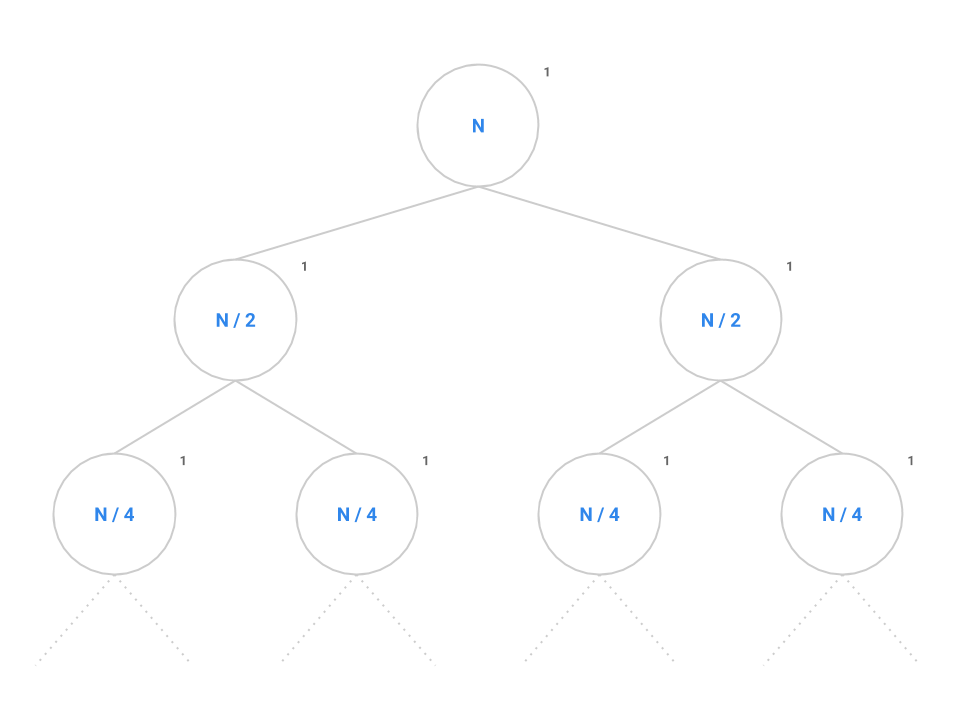
\includegraphics[scale=0.35]{images/02-bs-tree.png}
    \end{center}

    In each recursion step(level), we use 1 comparison(compare 
    $mid$ and $x$), then call recursion on a half 
    of the original array. From the image above, 
    we can easily notice there are total 
    $1+1+\cdots+1=1+\log_2 n$ comparisons.

    \section{Example: Towers of Hanoi}

    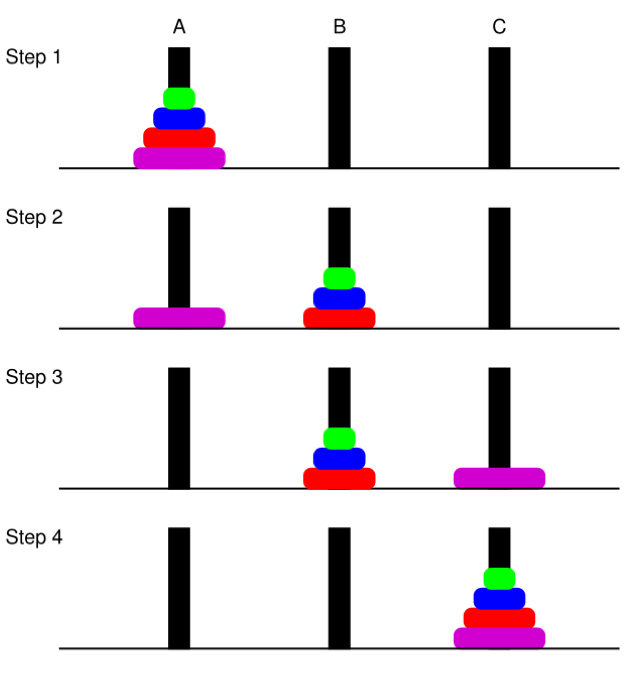
\includegraphics[scale=0.28]{images/02-hanoi.jpeg}
    
    In this example, we want to design an algorithm to 
    move all $n$ discs from peg $A$(start) to peg $C$(end), with the 
    constraints: (1) move one disc at a time, and 
    (2) cannot put larger disc on a smaller one.
    We are given another peg $B$(helper) where we can 
    temporary storage our discs.

    We still use the idea of {\bf Divide \& Conquer},
    consider how we can turn a problem of $n$ discs 
    into a problem of $n-1$? One possible solution is that,
    we can call recursion on upper $n-1$ discs, i.e., 
    move upper $n-1$ discs to peg $B$(helper peg), then move the remaining
    (the biggest) disc to peg $C$(end peg), and finally 
    move the $n-1$ discs from peg $B$(helper) to peg $C$(end).
    The following pseudocode shows this idea.

    \begin{algorithm}
        \caption{MoveTower($n$, $start$, $helper$, $end$)}
        \KwIn{$n$: num of discs}
        \eIf{$n=1$}{
            move the only disc from $start$ peg to $end$ peg

            return
        }{
            {\tcp {move first $n-1$ from $start$ peg to $helper$ peg}}
            {\tcp {so this time ``helper'' peg will be the old $end$ peg}}
            {\bf MoveTower($n-1$, $start$, $end$, $helper$)}

            move the only disc from $start$ peg to $end$ peg

            {\tcp {finally move first $n-1$ from $helper$ peg to $end$ peg}}
            {\tcp {this time ``helper'' peg will be the old $start$ peg}}
            {\bf MoveTower($n-1$, $helper$, $start$, $end$)}
        }
    \end{algorithm}

    Now we would like to analyze the time complexity of this algorithm,
    in other words, how many {\bf steps} are needed.
    Let $T(n)$ be the num of steps for $n$ discs, each time, 
    we first move $n-1$ disks from $start$ to $helper$, 
    costs $T(n-1)$ steps; then we move the biggest disk to $end$ peg,
    costs only 1 step; finally we move $n-1$ disks from $helper$
    to $end$, again costs $T(n-1)$ steps. To sum up:
    $$T(n)=2T(n-1)+1$$ when $n>1$, and $T(1)=1$.

    Now we solve the recurrence by the {\bf expansion method}:
    \begin{align*}
        T(n) &= 2T(n-1) + 1\\
             &= 2[2T(n-2)+1] + 1\\
             &= 4T(n-2)+3\\
             &= 4[2T(n-3)+1] + 3 \\
             &= 8T(n-3) + 7\\
             &= \cdots \\
             &= 2^i T(n-i) + (2^i-1)\\
             &= 2^{n-1} T(1) + (2^{n-1}-1)\\
             &= 2^n-1
    \end{align*}

    Or, with the recursion tree method:
    \begin{center}
        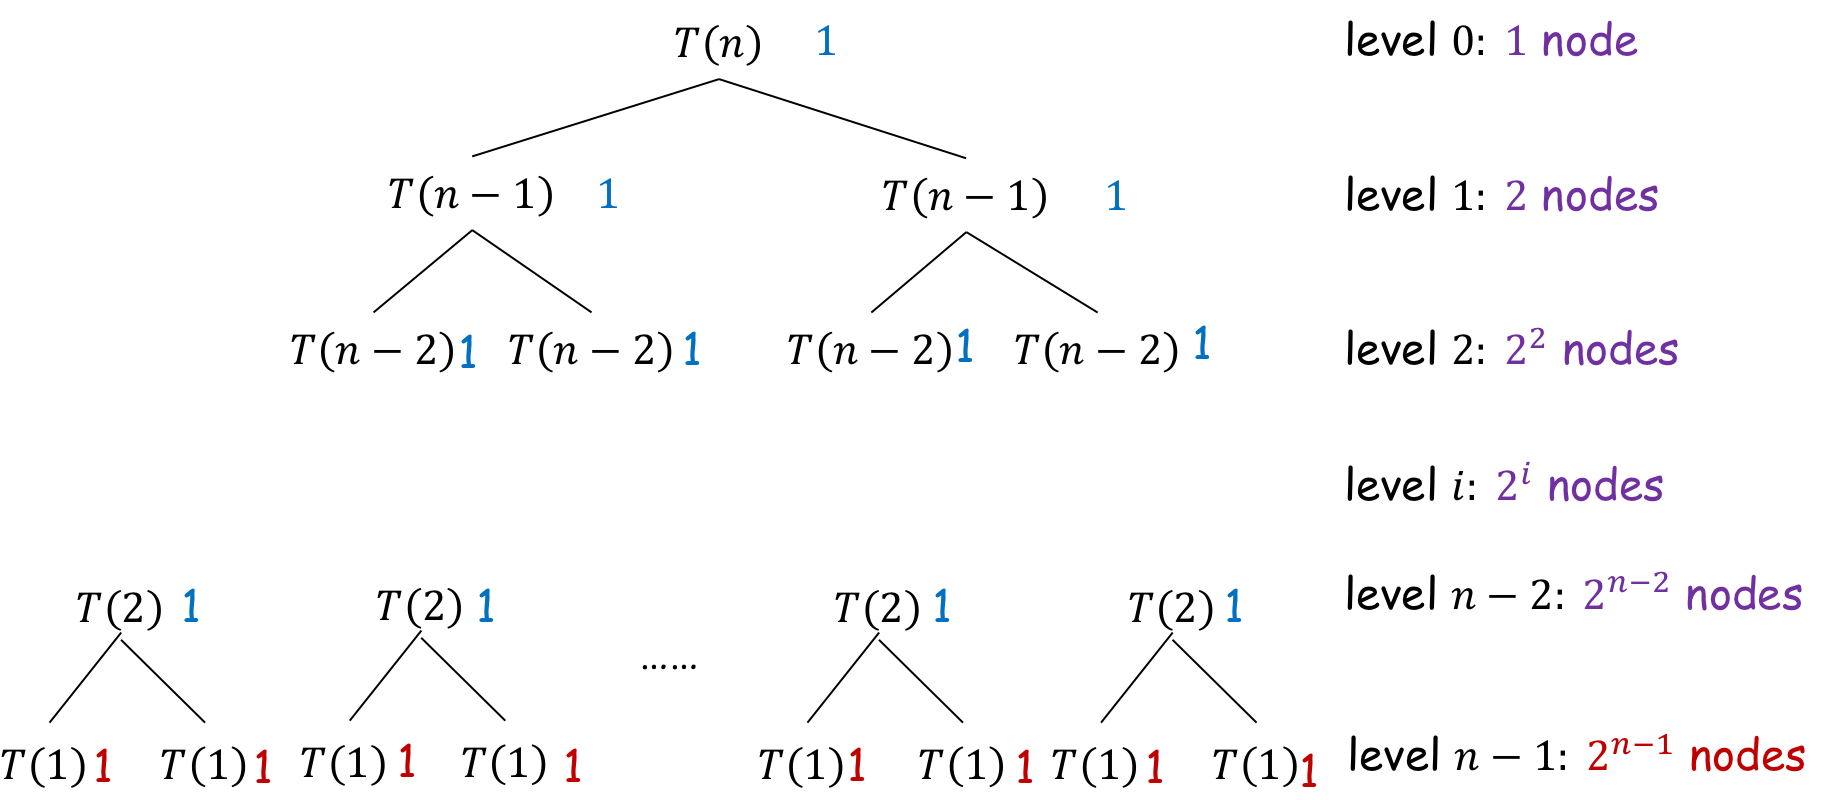
\includegraphics[scale=0.2]{images/02-hanoi-tree.jpeg}
    \end{center}
    
    There are, altogether, $1+2+2^2+2^3+\cdots + 2^{n-2}+2^{n-1}
    =2^n-1$ nodes, and we are doing one work(step) each node,
    then the time complexity is again, $2^n-1$.

    \section{Merge Sort}

    Now we again back to sorting, and we would like to introduce 
    a new algorithm or sorting: Merge Sort.
    This is a typical example of divide \& conquer, and 
    its process is like: (1) we first divide array into two halves,
    (2) then we recursively sort each half, (which means we 
    continuously divide it into halves, and then halves...)
    (3) finally {\bf merge} two halves to get a whole.

    The {\bf merge} operation may confuse you most. Here 
    it means combine two {\bf sorted lists} into a 
    whole sorted list. For example, given two sorted lists:
    $A=[2, 5, 7]$ and $B=[3, 4, 6, 10, 12]$, then after {\bf merge}
    operation, we will get $result=[2, 3, 4, 5, 6, 7, 10, 12]$.
    Since these two lists are sorted, we can do this process
    in $O(n)$ time, where $n$ is the length of result 
    list.(how many numbers in total) The basic idea is: 
    we compare the first item of $A$ and $B$, put the smaller 
    one, say, $A[1]$, in the first position of result list, then 
    we move on to the next item of $A$, but compare it still with 
    the {\bf first} item of $B$(since the first item of $B$
    has not yet inserted into result list), 
    and again put the smaller one into result list, then 
    continue move on. An example may help you understand the process:

    (1) Compare first items: $A=[{\blue 2},5,7], B=[{\blue 3},4,6,10,12]$, 
    $2<3$, so $result=[2]$;

    (2) then compare 2nd in $A$ and 1st in $B$, $A=[2, {\blue 5},7], B=[{\blue 3},4,6,10,12]$, 
    $3<5$, so $result=[2, 3]$;

    (3) continue the process, similarly, $A=[2, {\blue 5},7], B=[3,{\blue 4},6,10,12]$, 
    $4<5$, so $result=[2, 3, 4]$;

    (4) $A=[2, {\blue 5},7], B=[3,4,{\blue 6},10,12]$, 
    $5<6$, so $result=[2, 3, 4, 5]$;

    (5) $A=[2, 5,{\blue 7}], B=[3,4,{\blue 6},10,12]$, 
    $6<7$, so $result=[2, 3, 4, 5, 6]$;

    (6) $A=[2, 5,{\blue 7}], B=[3,4,6,{\blue 10},12]$, 
    $7<10$, so $result=[2, 3, 4, 5, 6, 7]$;

    (7) Now, all items in $A$ have already been inserted into result 
    list so that no items can be compared with items in $B$.
    Then we simply add remaining items in $B$ to result list,
    this will, obviously, ensure a sorted result list.(you may think of why)
    Hence $result=[2,3,4,5,6,7,{\blue 10,12}]$

    The pseudocode below shows the process:
    (below, append $\infty$ at the end of two lists can 
    free us from considering the situation that one list is 
    empty, like (7) above. Though different implementation, 
    the idea is entirely the same)
    
    \begin{algorithm}
        \caption{Merge($A$, $left$, $mid$, $right$)}
        \tcp{merge two sorted list: $A[left\cdots mid]$ and $A[mid+1\cdots right]$}
        $L\lar A[left\cdots mid],\ R\lar A[mid+1\cdots right]$

        append $\infty$ at the end of $L$ and $R$ \qquad \tcp{see explanation above}

        $i\lar 1,\ j\lar 1$\qquad  \tcp{two pointers point at items in $L$ and $R$}

        \For{$k\lar left$ {\rm to} $right$} {
            \tcp{always choose the smaller one to insert, and move on}
            \eIf{$L[i] \le R[j]$}{
                $A[k]\lar L[i]$

                $i\lar i + 1$
            }{
                $A[k] \lar R[j]$

                $j\lar j + 1$
            }
        }
    \end{algorithm}

    After learning how {\bf Merge} works, you now, hopefully,
    are able to understand how Merge Sort works, with the image below:

    \begin{center}
        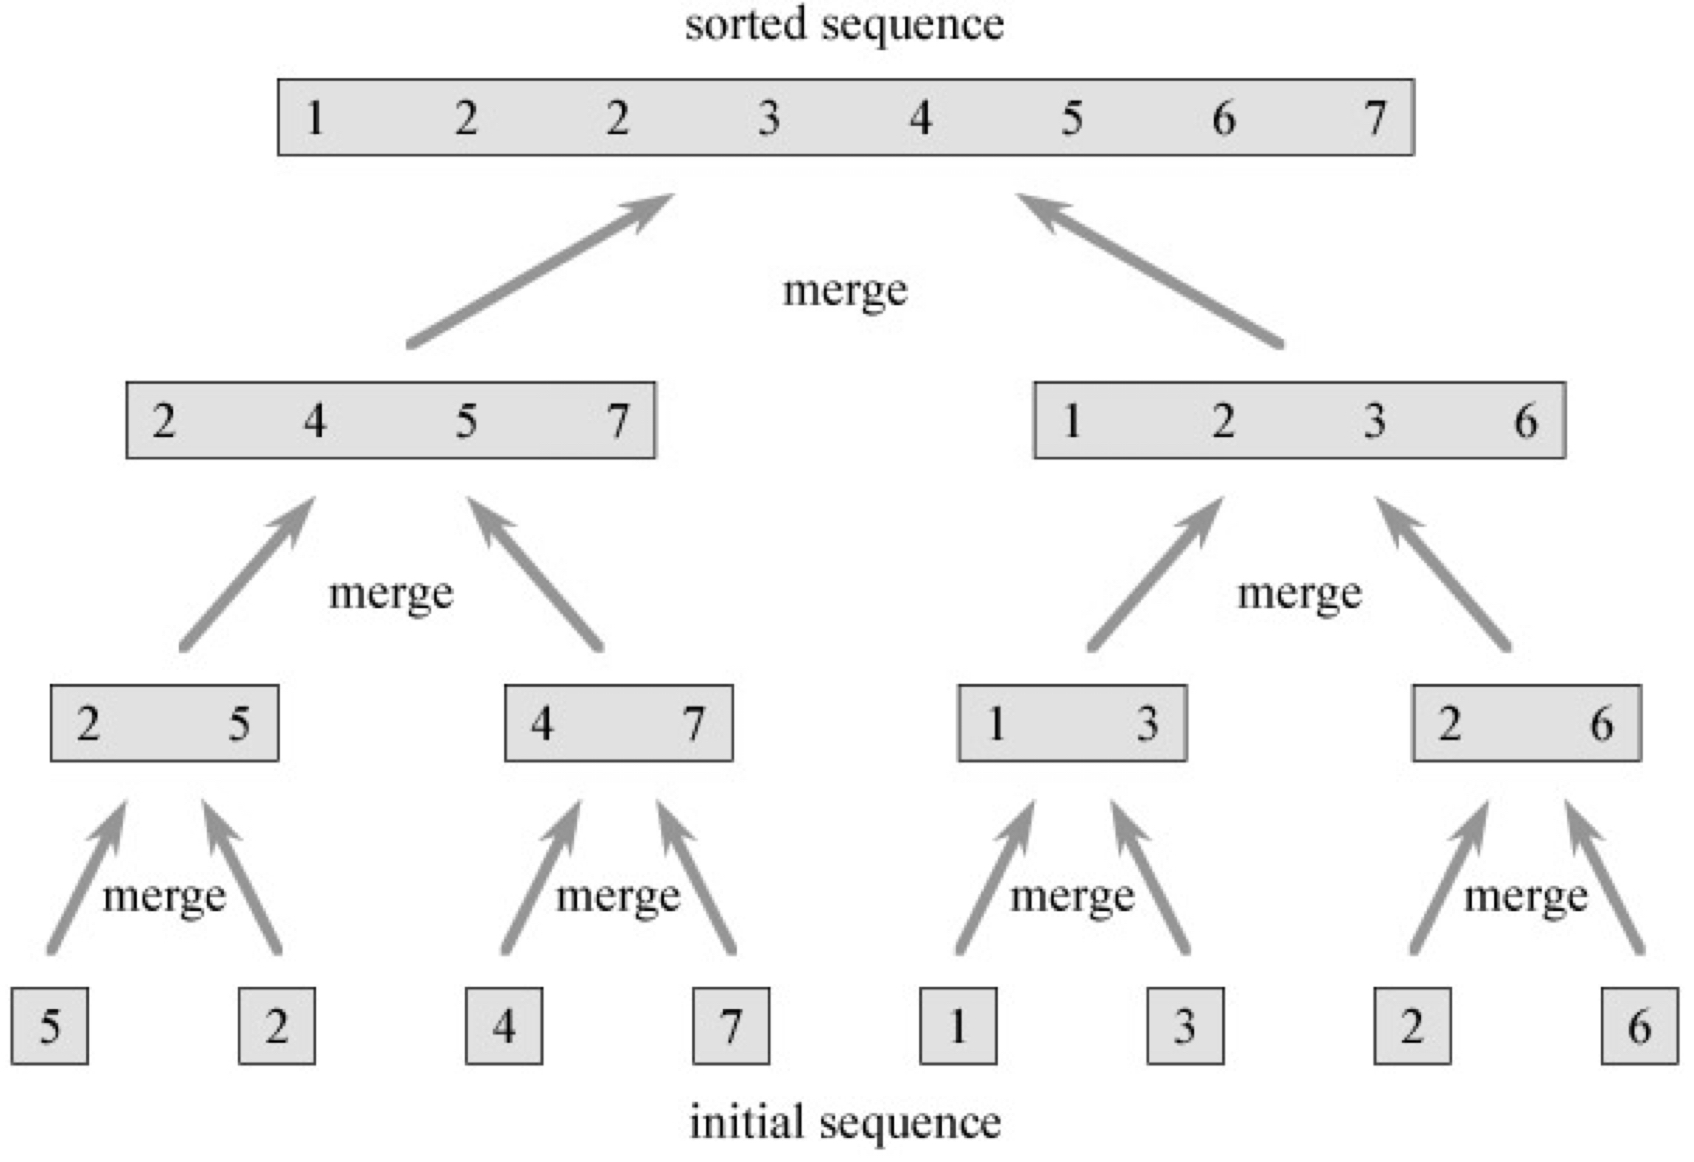
\includegraphics[scale=0.2]{images/02-mergeSort.jpeg}
    \end{center}
    
    We break down array recursively, until one element left,
    and then merge from bottom to up.
    The complete pseudocode for Merge Sort is given below:
    \begin{algorithm}
        \caption{MergeSort($A$, $left$, $right$)}
        \If{$left=right$}{return}
        $mid\lar \lfloor (left + right) / 2 \rfloor$

        \tcp{recursively divide array into two halves}

        {\bf MergeSort($A$, $left$, $mid$)}

        {\bf MergeSort($A$, $mid+1$, $right$)}

        \tcp{then merge from bottom to up}

        {\bf Merge($A$, $left$, $mid$, $right$)}
    \end{algorithm}

    Firstly call {\bf MergeSort($A$, 1, $n$)} to sort array $A$.
    
    As usual, we are interested in the running time of Merge Sort 
    algorithm. Let $T(n)$ be the running time on an array of size $n$,
    it's not hard to find 
    $T(n)\le T(\lfloor n/2 \rfloor) + T(\lceil n/2 \rceil)+O(n)$,
    when $n>1$ and $T(1)=O(1)$.

    Here we are actually able to simplify the equation. Firstly 
    we can replace $\le $ with $=$, since we are insterested
    in big-$O$ upper bound of $T(n)$; and with the same 
    reason, we can replace $O(n)$ with $n$, $O(1)$ with 1;
    finally, we can assume $n$ is a power of 2 for the sake of 
    simplicity but doesn't change the result at all, as 
    $T(n)\le T(n')\le T(2n)=O(T(n))$ where $n'$ is the 
    smallest power of 2 such that $n'\ge n$.

    Now we want to solve: 
    $T(n)=2T(n/2)+n$ for $n>1$, and $T(1)=1$.
    \begin{align*}
        T(n) &= 2\left(\frac{n}{2}\right)+n\\
             &= 2\left[ 2T\left(\frac{n}{4}\right) +\frac{n}{2}\right] + n
              = 2^2\cdot T\left(\frac{n}{2^2}\right) +2n\\
             &= 2^2\cdot \left[ 2T\left(\frac{n}{2^3}\right) +\frac{n}{2^2}\right] + 2n
              = 2^3\cdot T\left(\frac{n}{2^3}\right) +3n\\
             &= \cdots\\
             &= 2^{k}\cdot T\left(\frac{n}{2^k}\right) +kn
    \end{align*}
    We know the process ends with $\dfrac{n}{2^k}=1$ i.e. $k=\log_2 n$, thus
    \begin{align*}
        T(n) &= 2^{\log_2 n}T\left(\frac{n}{2^{\log_2 n}}\right)+n\cdot \log_2 n\\
             &= n\log_2 n+n
    \end{align*}
    In summary, merge sort runs in $O(n\log n)$ time.
    It is also worth pointing out that merge sort {\bf always}
    runs in $O(n\log n)$ time, which means best case is the same 
    as worst case, as you may think of it, 
    the complexity of merge sort {\it does not depend on inputs},
    it always break array down and then merge up.

    \section{Inversion Numbers}

    Given an array $A[1\cdots n]$, we say two elements $A[i]$ and $A[j]$
    are {\bf inverted} if $i<j$ but $A[i]>A[j]$, i.e., $A[i]$ appears
    before $A[j]$ but is larger than $A[j]$. The number of inverted pairs
    is called the {\bf inversion number} of array $A$. 
    Actually this is a useful measure, it provides us with an intuitive
    idea about how ``sorted'' an array is, larger inversion number implies
    a more unsorted array.

    What may surprise you is that inversion number has a close relation
    to insertion sort, and more concretely, {\bf the number of swaps
    used by insertion sort is equals to inversion number.}
    We can prove it by induction:
    
    \begin{proof}
        Assuming the array has size $n$. Basic case
        $n=2$ obviously holds.

        Inductive step: assume correct for an array of size $n-1$, i.e.,
        the total number of swaps performed while insertion sorting
        $A[1\cdots n-1]$ is equals to the inversion number of $A[1\cdots n-1]$.

        Let $x=A[n]$. Now, the remaining work by insertion sort is that we swap 
        $x$ with all items $A[j]$ such that $j<n$ and $A[j]>x$, 
        notice that the number of those items is the same of inversions in which
        {\bf $x$ participates}. Therefore, adding these new inversions gives
        the full inversion number of $A[1\cdots n]$.
    \end{proof}

    Now we will consider how to compute the inversion number of a given 
    array with size $n$. One possible method is we check all $(i,j)$
    pairs of given array, this requires ${n\choose 2}=\Theta(n^2)$
    running time. Another method uses the relation we proved above,
    running insertion sort and count the number of swaps we perform,
    but this also requires $\Theta(n^2)$ time since insertion sort 
    requires $\Theta(n^2)$. How can we improve that? 
    Come back to topic: divide and conquer!

    Similar to previous problems, we divide array into two halves, 
    and recursively count inversions in each half, but notice:
    we are missing something: we still need to count inversions
    where $a_i$ and $a_j$ are in different halves! We need 
    to return the sum of those three quantities finally.

    So the main problems is that, how we count the third quantity?
    Consider below situation, the two halves of array are:
    $[1,5,4,8,10,2]$ and $[6,9,12,11,3,7]$, how would you do that?
    You may count by hand, and knowing there are $5-3, 4-3, 8-6, \cdots$
    and in total 9 inversions with one item in 1st array and another in 
    2nd. But, it's really time consuming and totally a mess! We have 
    no efficient algorithm to do this but to count one by one.

    Fortunately, things will become much better if those two arrays are 
    {\it sorted}. For example, $A=[3,7,10,14,18,19]$ and 
    $B=[2,11,16,17,23,25]$. How will we do then? We can 
    scan progressively through both lists, and for each item 
    in $B$, we only need to find the smallest $A$ item 
    larger than it. In the lists above, for example, $A[1]=3$
    is larger than $B[1]=2$, so all items in $A$ form an inversion pair 
    with $B[1]$; then we move to $B[2]=11$, we try to find the smallest 
    item in $A$ larger than 11, so we move the pointer in $A$, 
    $A[2]=7<11, A[3]=10<11$, until $A[4]=14>11$, so 
    each item in $A[4]\cdots A[6]$ can form an inversion pair with $B[2]$.
    If we continue the process, we will finally get the inversion 
    number formed between $A$ and $B$, in $O(n)$ time. (Why is $O(n)$?
    Since we only iterate each item once during the whole process.
    You may find it quite similar to Merge operation in Merge Sort)

    \begin{algorithm}
        \caption{Count($A$, $l$, $mid$, $r$)}
        \tcp{
            $l$ means left, while $r$ means right.
        }

        \tcp{notice here, $L[1\cdots (mid-l+1)]$ is corresponding to 
        $A[l\cdots mid]$, the subscript changes, try not be confused later.
        $R$ also changes.}
        $L\lar A[l\cdots mid],\ R\lar A[mid+1\cdots r]$

        (here assume) $L, R$ already sorted

        $i\lar 1,\ j\lar 1$\qquad \tcp{two pointers for $L$ and $R$}

        $ans\lar 0$ \qquad \tcp{total inversion number}

        \tcp{let $i,j$ iterator over two arrays}
        \While{$i\le mid-l+1$ and $j\le r-mid$}{
            \tcp{looking for smallest $L$ item larger than $R$}
            \eIf{$L[i]\le R[j]$}{ 
                $i\lar i+1$
            }{
                \tcp{Found $L[i] > R[j]$!}

                \tcp{then $L[i]\cdots L[mid-l+1]$ each can form an inversion pair with $R[j]$,
                remind here $L$ subscript is diff from $A$, as stated above}

                \tcp{so inversion num for $R[j]$ is $mid-l+1-i+1=mid-l-i+2$}

                $inv\lar (mid-l-i+2)$

                $ans\lar ans+inv$

                $j\lar j+1$
            }
        }
        return $ans$
    \end{algorithm}

    And, the whole algorithm for counting the inversion number will be:

    \begin{algorithm}
        \caption{Count-Inversion($A$, $l$, $r$)}
        \If{$l=r$}{
            return 0
        }
        $mid \lar \lfloor (l+r)/2 \rfloor$

        $c_1\lar$ Count-Inversion($A$, $l$, $mid$)

        $c_2\lar$ Count-Inversion($A$, $mid+1$, $r$)

        MergeSort($A$, $l$, $mid$) 

        MergeSort($A$, $mid+1$, $r$) 

        $c_3\lar$ Count($A$, $l$, $mid$, $r$)

        return $c_1+c_2+c_3$
    \end{algorithm}

    First call: Count-Inversion($A$, 1, $n$).

    So far, you may think this is an excellent algorithm since we 
    only use $O(n)$ in each recursion step. However, it isn't! 
    Remember, we have assumed each half is already sorted, but in fact 
    they are random. If we firstly run some sort algorithm, say, 
    Merge Sort, and then do the counting above, the whole 
    running time will be:
    $$T(n)=2T(n/2)+\Theta (n\log n+n)=2T(n/2)+\Theta (n\log n)$$
    One can show $T(n)=\Theta(n\log^2 n)$.

    This is, to a certain degree, acceptable, compared to previous $\Theta(n^2)$,
    but we still want to improve that. 
    We can easily notice the main problem lies in sorting, which 
    uses $\Theta(n\log n)$ in each resursion step. How can we 
    reduce, or even avoid this process? 

    This is indeed hard to think about, but we can combine the sorting process 
    (more concretely, Merge sort)
    with the process which we count inversion pairs that form between the 
    two halves. In other words, previously we only do counting between 
    two halves, now we also perform Merge at the same time.
    What will this lead to? Consider from recursion bottom(1 item), 
    to top, each time we Merge the two halves, as what we did in 
    Merge Sort, and at the same time, count inversion pairs that cross 
    the two halves. And since we Merge from bottom to top, 
    the two halves will always be sorted.(this is exactly the same 
    Merge in Merge Sort)

    The paragraph above is still so abstract, at least for myself, 
    perhaps it's better to look at how the algorithm is implemented.\\

    \begin{algorithm}[H]
        \setstretch{1}
        \caption{Merge-and-Count($A$, $l$, $mid$, $r$)}

        \tcp{same as previous algorithm, subscripts for $L,R$ and $A$
        are different, remember this}

        $L\lar A[l\cdots mid],\ R\lar A[mid+1\cdots r]$

        append $\infty$ at the end of $L$ and $R$

        $i\lar 1,\ j\lar 1$ \qquad \tcp{two iteration pointers for $L$ and $R$}

        $count \lar 0$  \qquad \tcp{counter for inversion number}

        \For{$k\lar l$ to $r$}{
            \eIf{$L[i]\le R[j]$}{
                $A[k]\lar L[i]$

                $i\lar i+1$
            }{
                $A[k]\lar R[j]$

                $j\lar j+1$

                $count \lar count + (mid-l-i+2)$
            }
        }
        return $count$

    \end{algorithm}

    As you can find out above, apart from count inversion pairs 
    between $L$ and $R$, we merge them into a new array $A$,
    this is exactly what we did in merge sort, which maintains
    the ``sorted'' invariant. With the function above, 
    the complete algorithm for finding inversion number for an array is 
    displayed below.

    \begin{algorithm}
        \caption{Sort-and-Count($A$, $l$, $r$)}

        \If{$l=r$}{
            return 0
        }
        $mid\lar \lfloor (l+r)/2\rfloor$

        $c_1\lar $ Sort-and-Count($A$, $l$, $mid$)

        $c_2\lar $ Sort-and-Count($A$, $mid+1$, $r$)

        $c_3\lar $ Merge-and-Count($A$, $l$, $mid$, $r$)

        return $c_1+c_2+c_3$
    \end{algorithm}

    First call: Sort-and-Count($A$, 1, $n$)

    \section{The Maximum Subarray Problem}

    {\bf Problem:} Given an array of size $n$, the task is
    to find the largest possible sum of a contiguous subarray.
    For example, given $[3,2,1,-7,5,2,-1,3,-1]$, 
    subarray $[5,2,-1,3]$ has the largest sum among all subarrays,
    we need to output $5+2+(-1)+3=9$.

    We will provide a lot of algorithms to solve this problem.

    \subsection{brute force algorithm}

    The simplest idea is, for each pair $(i,j)$, we calculate
    $A[i]+A[i+1]+\cdots+A[j]$, and record maximum value 
    we have seen along the process.

    \begin{algorithm}
        \caption{Max-Subarray-Brute-Force($A$)}
        $maxSum \lar A[1]$ \qquad \tcp{can also use -inf to initialize}

        \For{$i\lar 1$ to $n$}{
            \For{$j\lar i$ to $n$}{
                \tcp{calculate $A[i]+\cdots+A[j]$}

                $sum\lar 0$

                \For{$k\lar i$ to $j$}{
                    $sum \lar sum + A[k]$
                }
                \tcp{if current $sum$ is larger, update $maxSum$}
                \If{$sum > maxSum$}{
                    $maxSum \lar sum$
                }
            }
        }
        return $maxSum$
    \end{algorithm}

    This is a very simple algorithm, but requires $\Theta(n^3)$ running time.

    \subsection{prefix sum}

    In brute force algorithm, we notice that each time when we 
    calculate $A[i]+A[i+1]+\cdots+A[j]$, we need to iterate through 
    these items, and add them together, which requires a lot of 
    redundant work. The {\bf prefix sum}, say $S[i]$, is defined 
    as $\sum_{j=1}^{i} A[i]$, i.e., the sum of all items before(and include)
    $A[i]$. If we have a table of all $S[i]$ values, we can now rewrite 
    $\sum_{k=i}^{j} A[k]=S[j]-S[i-1]$. See? That's a $\Theta(1)$ job!

    \vspace{0.2in}
    \begin{algorithm}
        \setstretch{1.5}
        \caption{Get-Prefix-Sum($A$)}
        \tcp{$S[]$ records the prefix sum of array $A$}
        $S[0]=0$

        \For{$i=1$ to $n$}{
            $S[i]\lar S[i-1]+A[i]$
        }
        return $S$
    \end{algorithm}

    \begin{algorithm}[H]
        \setstretch{1}
        \caption{Max-Subarray-Prefix-Sum($A$)}
        $maxSum \lar A[1]$ 

        $S\lar$ Get-Prefix-Sum($A$) \qquad \tcp{get prefix sum}

        \For{$i\lar 1$ to $n$}{
            \For{$j\lar i$ to $n$}{
                $sum\lar S[j]-S[i-1]$ \qquad \tcp{calculate $A[i]+\cdots+A[j]$}

                \If{$sum > maxSum$}{
                    $maxSum \lar sum$
                }
            }
        }
        return $maxSum$
    \end{algorithm}

    This reduces the running time of our algorithm to $\Theta(n^2)$.
    (Calculating prefix sum only requires $\Theta(n)$, 
    so overall $\Theta(n^2+n)=\Theta(n^2)$)

    \subsection{divide and conquer}

    Again, we return to our topic, and again, we try to cut 
    the array into two halves. Similar to {\bf Inversion Number}
    example, we classified all subarrays into three cases:
    \begin{enumerate}
        \item entirely in the first half
        \item entirely in the second half
        \item crosses the cut
    \end{enumerate}
    I think it will not surprise you that the third situation is 
    the most difficult one, while the first two cases, can still 
    be found recursively.

    \begin{algorithm}
        \caption{Max-Subarray-Divide-Conquer($A$, $l$, $r$)}

        \If{$l=r$}{return $A[l]$}

        $mid\lar \lfloor (l+r)/2 \rfloor$

        $max_1\lar $ Max-Subarray-Divide-Conquer($A$, $l$, $mid$)

        $max_2\lar $ Max-Subarray-Divide-Conquer($A$, $mid+1$, $r$)

        $max_3\lar $ Max Subarray that crosses the cut

        return $\max \{ max_1, max_2, max_3 \}$
    \end{algorithm}

    So how can we efficiently calculate $max_3$? Firstly, consider 
    what do we mean by ``crosses the cut''? That should be, 
    the subarray will {\it at least include both $A[mid]$ and $A[mid+1]$}
    in order to ``cross''. Hence these kind of subarray can always be 
    divided into two parts: $A[i\cdots mid]$ and $A[mid+1\cdots j]$
    for some $i$ and $j$. So in order to find max $A[i]+\cdots +A[j]$,
    we just find max $A[i]+\cdots +A[mid]$, and $A[mid+1]+\cdots +A[j]$,
    and finally add them together, this will definitely give us 
    the max value.

    Alright, so how can we find $i$?(and can use exactly the same 
    method to find $j$)
    It should be the index that maximize $A[i]+\cdots +A[mid]$.
    This is much easier since one end, say, $mid$, is fixed.
    We initialize $maxSum$ to $-\infty$, then scan from $mid$ towards left,
    each step we add an item to temporary $sum$, and update 
    $maxSum$ if $sum$ is larger. When we reach $l$(left end), 
    we will have already iterated all possible indices $i$ and 
    stored the max sum in $maxSum$.
    
    \begin{algorithm}
        \caption{Max-Subarray-Divide-Conquer($A$, $l$, $r$)}

        \If{$l=r$}{return $A[l]$}

        $mid\lar \lfloor (l+r)/2 \rfloor$

        $max_1\lar $ Max-Subarray-Divide-Conquer($A$, $l$, $mid$)

        $max_2\lar $ Max-Subarray-Divide-Conquer($A$, $mid+1$, $r$)

        \tcp{now let's count $max_3$}

        $L_m\lar -\infty,\ R_m\lar -\infty$

        $sum\lar 0$

        \For{$i=mid$ down to $l$}{
            $sum\lar sum + A[i]$

            \If{$sum > L_m$}{$L_m\lar sum$}
        }

        $sum\lar 0$

        \For{$i=mid+1$ to $r$}{
            $sum\lar sum + A[i]$

            \If{$sum > R_m$}{$R_m\lar sum$}
        }

        return $\max \{ max_1, max_2, L_m+R_m \}$
    \end{algorithm}

    First call {\bf Max-Subarray-Divide-Conquer($A$, 1, $n$)}.

    It's not difficult to find out the process of finding $max_3$
    requires $O(n)$ time, since we just scan throught the array.
    If let $T(n)$ be the running time of whole algorithm, 
    we will get:
    $$T(n)=2T(n/2)+O(n)$$
    This gives $T(n)=O(n\log n)$.

    \subsection{linear time?}

    Review the idea of calculating $max_3$ above, we said that 
    finding max $A[i]+\cdots +A[mid]$ is much easier since $mid$
    is a fixed ending point. This gives us an inspiration:
    for a {\it fixed} $j$, finding largest $A[i]+\cdots +A[j]=
    S[j]-S[i-1]$, is the same as finding the smallest $S[i-1]$
    .(Recall that $S[]$ is the prefix sum)
    If we can find the smallest $S[i-1]$ for each $j$,
    we will able to find the max subarray.(here $i-1$ must 
    be strictly smaller than $j$, otherwise the subarray is null)

    The process of finding smallest $S[i-1]$ can be easily done 
    during the iteration through array. More concretely, 
    we only need to update $minS = \min\{minS, A[i]\}$ at each step.
    Below shows the entire algorithm.
    
    \begin{algorithm}
        \caption{Max-Subarray-Linear($A$)}
        \tcp{Here we initialize $minS$ to 0 because {\it at least}
        we can do $S[j]-S[0]$ to ensure the sum is {\it at least}
        not smaller than $S[j]$}
        $maxSum \lar -\infty,\ minS\lar 0$

        \tcp{for each $j$, find $minS$, and then find $S[j]-minS$}
        \For{$j\lar 1$ to $n$}{
            \tcp{update overall answer}
            \If{$S[j]-minS>maxSum$}{
                $maxSum\lar S[j]-minS$
            }
            \tcp{update $minS$ so far}
            \If{$S[j] < minS$}{
                $minS\lar S[j]$
            }
        }
        return $maxSum$
    \end{algorithm}

    This algorithm can also be written without calculating prefix sum 
    before, since each time we only use $S[j]$, we only need one
    variable to record $S[j]$ and accumulate it each time.

    \begin{algorithm}
        \caption{Max-Subarray-Linear2($A$)}
        \tcp{$S$ will be all prefix sum so far, i.e., $A[1]+\cdots+A[j]$}
        $maxSum \lar -\infty,\ minS\lar 0,\ S\lar 0$

        \For{$j\lar 1$ to $n$}{
            $S\lar S+A[j]$ \qquad \tcp{calculate prefix sum so far}
            \If{$S-minS>maxSum$}{
                $maxSum\lar S-minS$
            }
            \tcp{update $minS$ so far}
            \If{$S < minS$}{
                $minS\lar S[j]$
            }
        }
        return $maxSum$
    \end{algorithm}

    As you can see, this algorithm only requires linear $\Theta(n)$ time.
    It is indeed a difficult progress that we optimize the algorithm 
    from $\Theta(n^3)$ down to $\Theta(n)$, with lots of new ideas 
    come out. We say this is ``More art than science''.

    \subsection{dynamic programming}

    By using {\bf dynamic programming} ideas, which we will formally 
    introduce later, we can also design quite efficient algorithms,
    but efficient always requires more thinking.
    Here we just give you a first taste on DP.

    We define $d[i]$ be the max sum of subarray that {\it 
    ends with $A[i]$}. Here we must contain $A[i]$ in 
    $d[i]$, otherwise, we cannot get $d[i+1]$ from $d[i]$,
    because it will break the ``consecutive'' subarray requirement.
    But if you ask me why we define in such a way, I cannot 
    explain it, and that is the ``art of dynamic programming'' :)

    So when we calculating $d[i]$, we only need to check $d[i-1]$
    and $A[i]$, this is the basic idea of dynamic programming, 
    that is, get value from previous values.
    And if $d[i-1]\le 0$, which means $d[i-1]+A[i]$ is not larger than 
    $A[i]$ itself! So why should we include $d[i-1]$ then, 
    we just let $d[i]=A[i]$, this will be the max sum with 
    $A[i]$ included.
    On the contray, if $d[i-1]>0$, then we should let 
    $d[i]=d[i-1]+A[i]$, since include $d[i-1]$ makes the sum 
    larger, and that is exactly what we want.

    \begin{algorithm}
        \caption{Max-Subarray-DP($A$)}
        $d[0]\lar 0$ \qquad \tcp{max sum of subarrays end with no item is 0}

        $maxSum\lar A[1]$\qquad \tcp{used to record max sum so far, notice here cannot initialize to 0}
        \For{$i=1$ to $n$}{
            \eIf{$d[i-1]\le 0$}{
                $d[i]\lar A[i]$
            }{
                $d[i]\lar d[i-1]+A[i]$
            }
            \If{$d[i]>maxSum$}{$maxSum=d[i]$}
        }
        return $maxSum$
    \end{algorithm}

    This is also a $\Theta(n)$ algorithm, and as usual, it is not easy 
    to think. But, we can still reduce the space it takes, i.e., 
    space complexity. Notice here we use an array $d[i]$ to record 
    the max sum of subarrays end with $A[i]$, but each time, 
    say, when we calculate $d[i]$, we only use the previous one,
    say, $d[i-1]$. So it is no need that we use an array to track this:
    we only need a variable to record the previous $d$ value,
    that's enough! So we can slightly modify the algorithm as below:

    \begin{algorithm}
        \caption{Max-Subarray-DP2($A$)}
        $previousD\lar 0$ 

        $maxSum\lar A[1]$

        \For{$i=1$ to $n$}{
            \eIf{$previousD\le 0$}{
                $previousD\lar A[i]$
            }{
                $previousD\lar previousD+A[i]$
            }
            \If{$previousD>maxSum$}{$maxSum=previousD$}
        }
        return $maxSum$
    \end{algorithm}

    \section{The Master Theorem}

    \subsection{Theorem and its proof}

    {\bf The Master Theorem:} Let $a\ge 1, b>1, c\ge 0$
    be constants, if $T(n)=aT(n/b)+n^d$, then:
    \begin{align*}
        \setstretch{0.7}
        T(n)=\left\{ \begin{array}{ll}
            O(n^d), & \text{if } d>\log_b{a}\\
            O(n^d\log n), & \text{if } d = \log_b{a}\\
            O(n^{\log_b{a}}), & \text{if } d < \log_b{a}\\
        \end{array}\right.
    \end{align*}

    There is one kind of proof given in lecture slide, 
    using expansion method. But personally, I like the method below.

    \begin{proof}
    Consider $T(n)=a\cdot T\left(\dfrac{n}{b}\right)+c\cdot n^{d}$,
    for the 0th layer of recursion(since we haven't begun recursion),
    running time is $c\cdot n^{d}$;
    for the 1st layer, there are $a$ branches, and each
    branch has running time $c\cdot \left(\dfrac{n}{b}\right)^d$, 
    in total $c\cdot \left(\dfrac{a}{b^d}\right)\cdot n^d$;
    for the 2nd layer, each branch in 1st layer has $a$ branches,
    so there are $a^2$ branches now, with each requires 
    $c\cdot \left(\dfrac{n}{b^2}\right)^d$, and 
    $c\cdot \left(\dfrac{a}{b^d}\right)^2\cdot n^d$ in total.
    We can easily find the pattern: 
    the running time of $k$-th layer is 
    $c\cdot \left(\dfrac{a}{b^d}\right)^k\cdot n^d$.

    Add all of them together, we get 
    $$T(n)=c\cdot n^d\cdot \left[ 1+ \left(\dfrac{a}{b^d}\right)+\cdots + \left(\dfrac{a}{b^d}\right)^k\right]$$

    Recall the sum of geometric sequence: 
    \begin{align*}
        \setstretch{0.7}
        1+p+p^2+\cdots +p^k=\left\{
        \begin{array}{ll}
            k+1, & \text{if } p=1\\
            \dfrac{p^{k+1}-1}{p-1}, & \text{if } p\ne 1
        \end{array}\right.
    \end{align*}
    Condition 1: when $a=b^d$, ratio is 1, so $T(n)=O(n^d\log n)$.

    Condition 2: when $a<b^d$, the sequence is decreasing, 
    so the sum is determined by the first item(you can also 
    infer from the equation of sum above), then $T(n)=O(n^d)$.

    Condition 3: when $a>b^d$, the sequence is increasing, 
    the sum is determined by the last item, this gives 
    $T(n)=n^{d}\left(\dfrac{a}{b^{d}}\right)^{\log _{b} n}=
    n^{d}\left(\dfrac{a^{\log _{b} n}}{\left(b^{\log _{b} n}\right)^{d}}\right)=
    a^{\log _{b} n}=
    \left(n^{\log_n{a}}\right)^{\log_b{n}}=
    n^{\left(\frac{\ln a}{\ln n}\cdot \frac{\ln n}{\ln b}\right)}=
    n^{\log _{b} a}$.
    \end{proof}

    \subsection{equalities, inequalities and more}

    {\Large\color{red} to be added. (2021/09/05)}

    \section{Integer Multiplication}

    You may first think of using primary school method: 
    i.e., ``long multiplication'', and this requires $\Theta(n^2)$
    time. We will show that we can do better than this, but 
    the ideas are quite difficult to think of, and actually 
    people used quite a long time to invent the algorithms.

    \subsection{divide and conquer: first attempt}

    For example, we would like to calculate $3711\times 4021$,
    we can divide each number into two parts: {\bf high} part 
    and {\bf low} part, say, $x_h=37, y_h=40$, and $x_l=11, y_l=21$.
    Then, $x\times y=x_h\times y_h\cdot 10^n+(x_l\times y_h+x_h\times 
    y_l)\cdot 10^{n/2}+x_l\times y_l$, where $n$ is the length of 
    two numbers. One thing worths mentioning is that we can always 
    take $n$ as a perfect square of 2, and if it is not, we just 
    put some 0s in front of the number.
    So now, there are four multiplications and we can use recursion 
    to calculate each of them. And for multiplying power of 10, 
    we can just think of it as adding some 0s after the number, so 
    this takes $O(n)$ time.

    \begin{algorithm}
        \caption{multiply-DC($A$, $B$)}
        \tcp{$A[1\cdots n]$ and $B[1\cdots n]$ are two arrays storing 
        string of base 10. $A[1], B[1]$ are least siginificant bits.(LSB)}

        $n\lar $ size of $A$ and $B$

        \If{$n=1$}{return $A[1]\cdot B[1]$}

        $mid\lar \lfloor n/2 \rfloor$

        $M_1\lar $multiply-DC($A[mid+1\cdots n]$, $B[mid+1\cdots n]$)
        \qquad \tcp{$x_h\times y_h$}

        $M_2\lar $multiply-DC($A[1\cdots mid]$, $B[mid+1\cdots n]$)
        \qquad \tcp{$x_l\times y_h$}

        $M_3\lar $multiply-DC($A[mid+1\cdots n]$, $B[1\cdots mid]$)
        \qquad \tcp{$x_h\times y_l$}

        $M_4\lar $multiply-DC($A[1\cdots mid]$, $B[1\cdots mid]$)
        \qquad \tcp{$x_l\times y_l$}

        \tcp{Below we can put numbers in array directly, or 
        append 0 at the end and add them together.
        Assume $res[]$ is filled with 0 at the beginning.}

        $res[1\cdots n]\lar M_4$

        $res[mid+1\cdots ]\lar res[mid+1\cdots] + M_2+M_3$

        $res[n+1\cdots]\lar res[n+1\cdots]+M_1$

        return $res$
    \end{algorithm}

    This will require a running time as $T(n)=4T(n/2)+O(n)$, 
    hence $T(n)=O(n^2)$, which doesn't improve our algorithm 
    at all. One may think of using binary representation(base 2)
    instead of decimal, but this doesn't help either, 
    though multiply by power of 2 can be done in $O(1)$ time, 
    with the help of left shift($<<$), write the result into 
    the array still takes $O(n)$, regardless of the time 
    converting an integer of base 10 into base 2. 
    So basically, we need to reduce the time we call recursion 
    to reduce the running time.

    \subsection{Karatsuba's method}

    As shown above, we need to calculating 4 multiplications,
    which makes us to call 4 recursions. Trying to improve that, 
    Karatsuba noticed that we only need $x_h\times y_l+x_l\times y_h$(the sum),
    instead of calculating each of the multiplication result.
    He suggested we only need to calculate 3 times, and they are:
    $M_1=x_h\times y_h, M_2=x_l\times y_l, M_3=(x_h+x_l)\times 
    (y_h+y_l)$, then we can get $x_h\times y_l+x_l\times y_h$ 
    by doing $M_3-M_1-M_2$. This successfully reduce the 
    running time of multiplication algorithm, with only 3 
    recursion calls:
    $T(n)=3T(n/2)+O(n)$, gives $T(n)=n^{\log_2 3}\approx n^{1.585}$.

    \begin{algorithm}
        \caption{Karatsuba($A$, $B$)}
        \tcp{$A[1\cdots n]$ and $B[1\cdots n]$ are two arrays storing 
        string of base 10. $A[1], B[1]$ are LSB.}

        $n\lar $ size of $A$ and $B$

        \If{$n=1$}{return $A[1]\cdot B[1]$}

        $mid\lar \lfloor n/2 \rfloor$

        $M_1\lar $Karatsuba($A[mid+1\cdots n]$, $B[mid+1\cdots n]$)
        \qquad \tcp{$x_h\times y_h$}

        $M_2\lar $Karatsuba($A[1\cdots mid]$, $B[1\cdots mid]$)
        \qquad \tcp{$x_l\times y_l$}

        $A'\lar A[mid+1\cdots n]+A[1\cdots mid]$

        $B'\lar B[mid+1\cdots n]+B[1\cdots mid]$

        $M_3\lar $Karatsuba($A'$, $B'$)
        \qquad \tcp{$(x_h+x_l)\times (y_h+y_l)$}

        \tcp{Assume $res[]$ is filled with 0 at the beginning.}

        $res[1\cdots n]\lar M_2$

        $res[mid+1\cdots ]\lar res[mid+1\cdots] +M_3-M_1-M_2$

        $res[n+1\cdots]\lar res[n+1\cdots]+M_1$

        return $res$
    \end{algorithm}

    \subsection{So far...}

    Inspired by Karatsuba, people can improve his algorithm by 
    ``dividing each integer into 3 parts, and solve 5 multiplications'',
    or ``divide into $n$ parts, and solve $2n-1$ multiplications'' etc.
    Later on, in 1971, Strassen solved this problem in 
    $O(n\log n\log \log n)$, using {\bf Fast Fourier Transformation(FFT)}.
    In 2007, $O(n\log n\cdot 8^{\log ^* n})$ algorithm was found 
    and in 2019, finally, $O(n\log n)$ algorithm was found.

    However, Karatsuba's algorithm isn't always faster than 
    our primary school $O(n^2)$ method, since it has a larger 
    constant. In practice, people find that for integers with
    length less than 20, using our $O(n^2)$ method is better;
    while Karatsuba's algorithm is better for length $20\sim 2000$,
    FFT is better for $>2000$. And for your reference, Python 
    uses 70 as a critical value to judge whether to perform 
    primary school method or Karatsuba's method.

    \section{Matrix Multiplication}

    Given two $n\times n$ matrices $A, B$, how can we compute 
    $C=AB$?
    
    Since $c_{ij}=\sum_{k=1}^{n}a_{ik}b_{kj}$, 
    we can use three nested loops to calculate each items in $C$,
    in $\Theta(n^3)$ time. This is our brute force algorithm.

    \subsection{divide and conquer?}

    Much similar to integer multiplication, we try to divide 
    $A$ and $B$ into $\frac{1}{2}n\times \frac{1}{2}n$ matrices 
    and call recursion to multiply each part.
    \begin{align*}
        \setstretch{0.5}
        \left[ \begin{array}{cc}
            C_{11} & C_{12} \\
            C_{21} & C_{22}
        \end{array} \right]
        =
        \left[ \begin{array}{cc}
            A_{11} & A_{12} \\
            A_{21} & A_{22}
        \end{array} \right]
        \left[ \begin{array}{cc}
            B_{11} & B_{12} \\
            B_{21} & B_{22}
        \end{array} \right]
    \end{align*}
    and,
    \begin{align*}
        C_{11} &= (A_{11}\times B_{11}) + (A_{12}\times B_{21}) \\
        C_{12} &= (A_{11}\times B_{12}) + (A_{12}\times B_{22}) \\
        C_{21} &= (A_{21}\times B_{11}) + (A_{22}\times B_{21}) \\
        C_{22} &= (A_{21}\times B_{12}) + (A_{22}\times B_{22}) 
    \end{align*}
    This algorithm requires $T(n)=8T(n/2)+O(n^2)$, notice 
    here add matrices is $O(n^2)$. We can easily know 
    $T(n)=O(n^3)$, from Master's Theorem.

    \subsection{Strassen's method}

    This is not easy to improve. But inspired by integer multiplication,
    Strassen managed to calculate that with only 7 multiplications:
    \begin{center}
        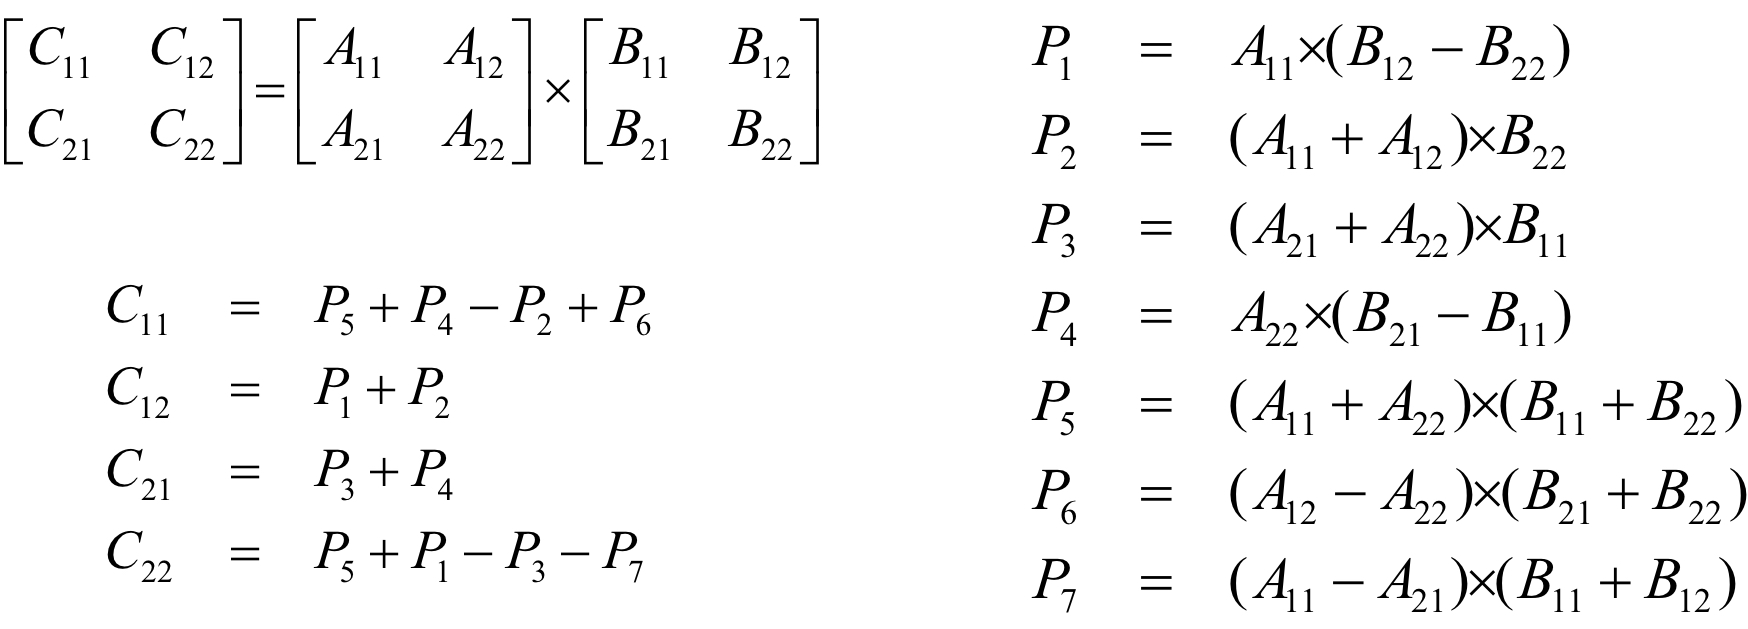
\includegraphics[scale=0.23]{images/02-matrix-mult.jpg}
    \end{center}
    
    And this reduce the running time down to 
    $O(n^{\log_2 7})\approx O(n^{2.807})$.

    Again, many people are trying to reduce the time complexity 
    and another competition arose. 
    We would not go into details here.

    {\it This is the end of class note. Last modified: Sep 05, 2021.}


\end{spacing}
\end{document}
